\documentclass[sigconf, authordraft]{acmart}
\usepackage[linesnumbered]{algorithm2e}
\usepackage[format=plain, labelfont={bf}, textfont=normal]{caption}
\usepackage{booktabs,xcolor}
\begin{document}
\title{GPU-friendly Stroke Expansion}
\author{Raph Levien}
\author{Arman Uguray}
\affiliation{
    \institution{Google}
    \city{San Francisco}
    \state{CA}
    \country{USA}
}

\begin{abstract}
    Vector graphics includes both filled and stroked paths as the main primitives. While there are many techniques for rendering filled paths on GPU, stroked paths have proved more elusive. This paper presents a technique for performing stroke expansion, namely the generation of the outline representing the stroke of the given input path. Stroke expansion is a global problem, with challenging constraints on continuity and correctness. Nonetheless, we implement it using a fully parallel algorithm suitable for execution in a GPU compute shader, with minimal preprocessing. The output of our method can be either line or circular arc segments, both of which are well suited to GPU rendering, and the number of segments is minimal. We introduce several novel techniques, including an encoding of vector graphics primitives suitable for parallel processing, and an Euler spiral based method for computing approximations to parallel curves and evolutes.
\end{abstract}

\maketitle
\thispagestyle{empty}
\pagestyle{plain}

\section{Introduction}

Rendering of vector graphics documents requires handling both filled and stroked primitives. There is substantial literature on GPU rendering of filled paths, but many fewer published techniques for strokes. It is a more challenging problem, especially for parallel computation, because path segments cannot be processed independently of each other; the \emph{joins} between adjacent path segments depend on context. In addition, the path topology affects the rendered result, in particular whether subpaths are open or closed. In the former case, the endpoints are rendered with \emph{caps}. Joins and caps can have multiple styles, including different styles within the same document.

Stroke expansion is the process of generating an outline that, when filled, produces the \emph{stroke} of a given input path. Informally, a line of the same width as the stroke is swept along the path, normal to it, and also decorated with joins and caps. Though stroke rendering is referenced in many 2D graphics standards, it has lacked a precise formal definition until recent work, primarily \cite{Nehab2020} and \cite{Kilgard2020}.

The \cite{Nehab2020} paper gives a comprehensive survey of techniques for stroke expansion, and an algorithm which, for a number of reasons, is only suitable for implementation on CPU (though adapting it to GPU is listed as promising future work). It classifies techniques into \emph{local,} where each path segment generates closed geometry (which may be triangles or other primitives), and \emph{global,} where the overall result is a closed outline of the stroked path, but the partial result from each segment is in general open. Our technique is considered global in this scheme, yet allows independent processing of each path segment.

A number of factors contribute to an algorithm being ``GPU-friendly.'' In addition to simply being able to process the input segments in parallel, such an algorithm also avoids divergent control flow (avoiding the need for explicit subdivision at special events such as inflection points and cusps) and uses robust numerical techniques not subject to particular problems when evaluated using 32-bit floating point numbers.

We propose that the correctness of stroke outlines be divided into \emph{weak correctness} and \emph{strong correctness.} We define strong correctness as the computation of the outline of a line swept along the segment, maintaining normal orientation, combined with stroke caps and joins. Weak correctness, by contrast, only requires the parallel curves of stroke segments, combined with caps and the outer contours of joins. The two notions are equivalent for sufficiently well-behaved input, in particular when the curvature measured at endpoints of path segments does not exceed the reciprocal of the half linewidth. As described in detail in \cite{Nehab2020}, very few existing implementations actually implement the strong version, so document authors have become accustomed to not depending on behavior at endpoints. Standards for graphics formats, such as SVG\cite{Svg2}, also provide an ``out,'' enabling the weaker behavior. While our current implementation emphasizes weak correctness, we believe it can be extended to the stronger sense, by implementing evolutes and inner join contours.

A great number of rendering techniques for strokes have been proposed. Some are \emph{local,} in that they break the stroke up into smaller closed pieces, the union of which forms an approximation to the stroke. Included in this category is polar stroking \cite{Kilgard2020}, which proposes a GPU-friendly subdivision scheme based on an angle step error. Others are based on stroke expansion, generating an explicit outline, which is then filled to produce the stroke rendering. Such techniques are further divided into \emph{flattening} approaches, where the outline is approximated by a polyline, and \emph{curve-based} approaches, exemplified by the approach in \cite{Nehab2020}. In both cases, the outline contains approximations of parallel curves of the input curve segments, and, as proposed in \cite{Nehab2020}, their evolutes when targeting strong correctness. For a more detailed survey of existing stroke rendering techniques, the reader is directed to Section 4 of \cite{Nehab2020}.

The subproblem of approximating parallel curves has also spawned extensive literature, none of which is entirely satisfying, especially when it comes to algorithms that can be efficiently evaluated on GPU. An example of a reasonably good algorithm that computes flattened parallel curves is \cite{Yzerman2020}, as used in the Blend2D rendering library. For producing curved outlines, the Tiller and Hanson algorithm\cite{Tiller1984} is commonly implemented and cited, but its performance is quite poor when applied to cubic Béziers. The quadratic Bézier version is adequate, and forms the basis of the algorithm in \cite{Nehab2020}. A variant is also used in Skia\cite{Skia}; instead of lowering the cubic Bézier to a quadratic approximation and then computing the parallel curve, Skia approximates the parallel curve directly with a quadratic Bézier, then measures the error to determine whether further subdivision is necessary.

This paper presents a comprehensive solution to stroke expansion, well suited to GPU implementation. It can produce both flattened polylines or an approximation consisting of circular arcs. The best choice depends on the capabilities of the path rendering mechanism following stroke expansion, but as we show, outlines consisting of circular arcs have many fewer segments and are correspondingly faster to produce. The algorithm is based on Euler spiral segments as an intermediate representation, with an iterative algorithm based on a straightforward error metric for conversion from cubic Béziers. We have also devised a compact binary encoding of paths, suitable for fully parallel computation of stroke outlines, while requiring minimal CPU-side processing. Our algorithm has been implemented in GPU compute shaders, integrated in a full rendering engine for vector graphics, and shows a dramatic speedup over CPU methods.

\section{Flattening and arc approximation of curves}

% Note: this is being written as a fairly stand-alone section. No doubt some reorganization should happen

The core problem in stroke expansion is approximating the desired curve by segments of some other curve, usually a simpler one. These segments must be within an error tolerance of the source curve, and ideally close to a minimal number of them. We consider a number of source to target pairs, most importantly cubic Béziers to Euler spirals, and Euler spiral parallel curves to either lines or arcs.

There are generally three approaches to such curve approximation. The most straightforward but also least efficient is ``cut then measure,'' usually combined with adaptive subdivision. In this technique, a candidate approximate curve is produced, then the error is measured against the source curve, usually by sampling a number of points along both curves and determining a maximum error (or perhaps some other error norm). If the error is within tolerance, the approximation is accepted. Otherwise, the curve is subdivided (usually at $t = 0.5$) and each half is recursively approximated. A substantial fraction of all curve approximation methods in the literature are of this form, including \cite{Nehab2020}. The main disadvantage is the cost of computing the error metric. Another risk is underestimating the error due to inadequate sampling; this is a particular problem when the source curve contains a cusp.

% Note: would be cool to run profiler on Nehab code to determine fraction of time computing error metric.

The next approach is similar, but uses an \emph{error metric} to estimate the error. Ideally such a metric is a closed-form computation rather than requiring iteration. A good error metric is conservative, yet tight, in that it never underestimates the error (which would allow results exceeding the error bound to slip through), and does not significantly overestimate the error, which would result in more subdivision than optimal.

By far the most efficient approach is an \emph{invertible} error metric. In this approach, the error metric has an analytic inverse, or at least a good numerical approximation. Because the metric is invertible, it can predict the number of subdivisions needed, as well as the parameter value for each subdivision. If the error metric is accurate, then approximation is near-optimal. One example of an invertible error metric is angle step, used in polar stroking\cite{Kilgard2020}; the number of subdivisions is the total angle subsumed by the curve divided by the angle step size, and the parameter value for each subdivision is the result of solving for a tangent direction. Another widely used invertible error metric is Wang's formula (\cite{Goldman2003}, Section 5.6.3), which gives a bound on the flattening error based on the second derivative of the curve. This metric is conservative but works well in practice; among other applications, it is used in Skia for path flattening. One limitation of Wang's method is that it only applies to the flattening of filled outlines; when applied naively to generation of parallel curves, it can undershoot substantially, especially near cusps.

% Note: an alternate cite for the central result of Wang's formula is Sederberg's lecture notes. It doesn't use the name "Wang's formula." In one way, it is a cleaner result, as it doesn't have the rounding up to a power of 2. But it is also less of an archival cite.
% https://scholarsarchive.byu.edu/cgi/viewcontent.cgi?article=1000&context=facpub#section.10.6

\subsection{Error metrics for flattening}

The distance between a circular arc segment of length $s$ and its chord, with angle between arc and chord of $\theta$ (see Figure~\ref{fig:arc_chord}), is exactly $(1-\cos \theta)\frac{s}{2\theta}$. The curvature is $\kappa = \frac{2\theta}{s}$ (equivalently, $\theta = \frac{\kappa s}{2}$), and this remains constant even as the arc is subdivided. Rewriting, $d = (1-\cos\frac{\kappa s}{2})\frac{1}{\kappa}$. From this, we can derive a precise, invertible error metric. Subdividing the arc in to $n$ segments, the distance error for each segment is $\frac{1}{\kappa}(1-\cos \frac{\kappa s}{2n})$. Solving for n, we get:

\begin{figure}
    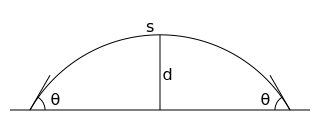
\includegraphics[scale=0.5]{arc_chord}
    \caption{A circular arc segment with notations for angles ($\theta$), arc length ($s$), and distance to chord ($d$)}
    \Description{A circular arc above its chord, with labels at the endpoints for angle from chord ($\theta$), the length of the arc ($s$) and the maximum distance from the arc to its chord ($d$).}
    \label{fig:arc_chord}
\end{figure}

% TODO: I might supplement this figure with one subdivided with n=3

\[
n = \frac{s\kappa}{2\cos^{-1}\left( 1- d\kappa \right)}
\]

To flatten a finite arc, round up $n$ to the nearest integer. This will cause the error to decrease, so will still be within the error bounds.

Note that the number of subdivisions is proportional to the arc length. Another way of stating this relationship is that the \emph{subdivision density}, the number of subdivisions per unit of arc length, is constant.

The error metric for flattening an arc is exact. It always yields the minimum number of subdivisions needed to flatten the curve, and the flattening error is the least possible with given that number of subdivisions. For general curves, an exact error bound is not feasible, and we resort to an approximation. Again the circular arc provides a good example. Applying the small angle approximation $\cos \theta \approx 1 - \theta^2/2$, the approximate distance error is $d = \frac{\kappa s^2}{8n^2}$, and solving for $n$ we get $n = s\sqrt{\frac{\kappa}{8d}}$. Note that this estimate is \emph{conservative,} in that it will always request more subdivision and thus produce a lower error than the exact metric.

We are of course concerned with the flattening of more general curves (ultimately the parallel curve of a cubic Bézier), not simply circular arcs. It is tempting to sample the curvature and plug it into the formula above, but this can both dramatically undershoot the error (predicting that no subdivision is needed at an inflection point) and overshoot it (requiring infinite subdivision at a cusp; and cusps). Apparently, some kind of average curvature is needed.

We propose the following error metric to estimate the maximum distance between an arbitrary curve of length $\hat{s}$ and its chord. 

\[
    d \approx \frac{1}{8}\left(\int_0^{\hat{s}} \sqrt{|\kappa(s)|}ds \right)^2
\]

% Should s-hat be the integration variable instead? Is there a better choice of symbol?

This formula is the same as the approximate error metric for circular arcs, except that instead of a constant curvature value, a norm-like average with an exponent of 1/2 is used (it is not considered a true norm because the triangle inequality does not hold). We chose this particular formulation because it tends to produce invertible error metrics, and because it works well in practice.

This formula also has a meaningful interpretation: the quantity under the integral sign is the subdivision density, and represents the number of subdivisions per unit length of an optimal flattening as the error tolerance approaches zero. In particular, the number of subdivisions is:

\[
    n = \left(\int_0^{\hat{s}} \sqrt{|\kappa(s)|}ds \right)\sqrt{\frac{1}{8d}}
\]

In addition, if the function represented by the integral is invertible, then the corresponding error metric is invertible. Evaluate the function to determine the number of subdivision points, then evenly divide the result, using the inverse of the function to map these values back into parameter values for the source curve being approximated.

\subsection{Error metrics for flattening Euler spirals}

We choose Euler spiral segments for our intermediate curve representation precisely because their simple formulation in terms of curvature (Cesàro equation) results in similarly simple subdivision density integrals.

An Euler spiral segment is defined by $\kappa(s) = as+b$, or alternatively $\kappa(s) = a(s-s_0)$, where $s_0 = -b/a$ is the location of the inflection point. Applying the above error metric, the subdivision density is simply $\sqrt{|a(s-s_0)|}$. The integral is $\frac{2}{3}\sqrt{a}(s-s_0)^{1.5}$, which is readily invertible.

An immediate consequence is that flattening an Euler spiral by choosing subdivision points $s_i = a\cdot i^\frac{2}{3}$ produces a near-optimal flattening, as can visually be seen in Figure~\ref{fig:es_flatten}.

\begin{figure}
    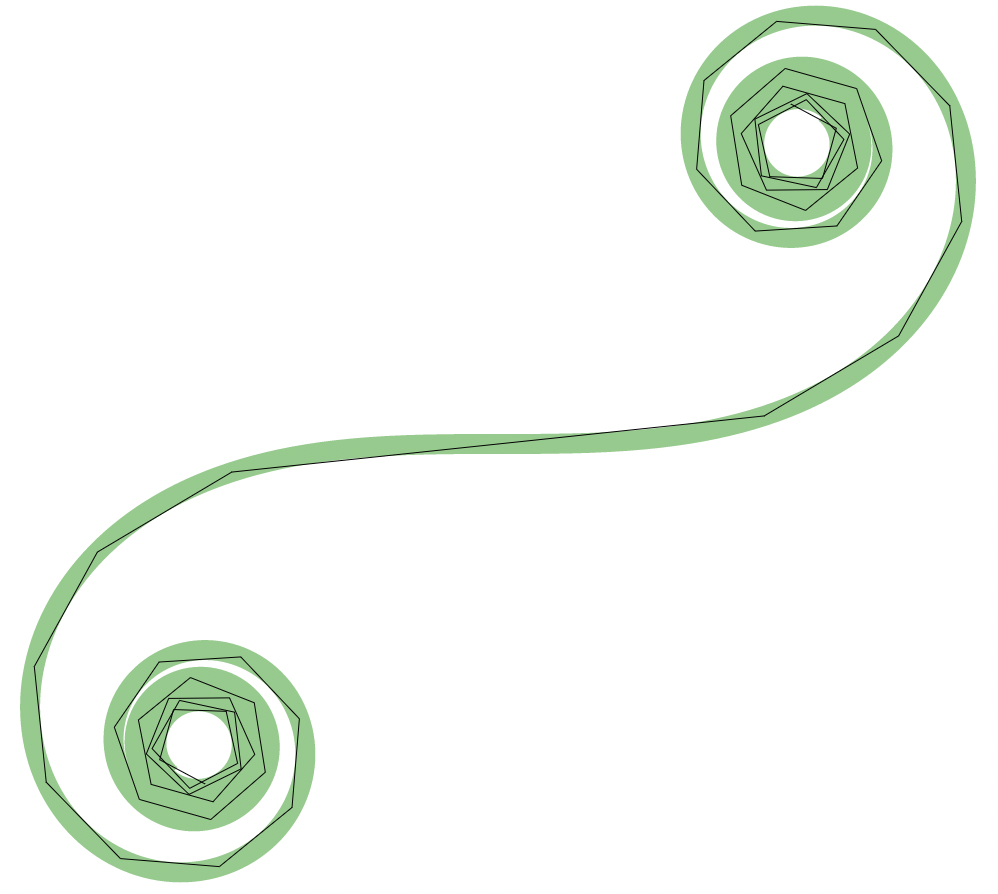
\includegraphics[scale=0.3]{es_flatten}
    \caption{Flattening of an Euler spiral using points spaced by power-law}
    \Description{An Euler spiral along with its flattened representation. The flattened curve has an error}
    \label{fig:es_flatten}
\end{figure}


\section{Euler spirals and their parallel curves}

It is common to approximate cubic Béziers to some intermediate curve format more conducive to offsetting and flattening. A number of published solutions (\cite{Yzerman2020}, \cite{Nehab2020}) use quadratic Béziers, as it is well suited for computation of parallel curves. Even so, this curve has some disadvantages. In particular, it cannot model an inflection point, so the source curve must be subdivided at inflection points.

Like these other approaches, we also use an intermediate curve, but our choice is an Euler spiral. In some ways it is similar to quadratic Béziers -- it also has $O(n^4)$ scaling and is best computed using geometric Hermite interpoliation -- but differs in others. It has no difficulty modeling an inflection point. Further, its parallel curve has a particularly simple mathematical definition and clean behavior regarding cusps.

An Euler spiral segment is defined as having curvature linear in arc length.

The parallel curve of the Euler spiral (also known as ``clothoid'') was characterized by Wieleitner well over a hundred years ago\cite{Wieleitner1907}, and has a straightforward closed-form Cesàro representation, curvature as a function of arc length. TODO: present closed-form solution.

\section{Flattened parallel curves}

The geometry of a stroke outline consists of joins, caps, and the two parallel curves on either side of the input path segemnts, offset by the half linewidth. The former are not particularly difficult to calculate, but parallel curves of cubic Béziers are notoriously tricky. Analytically, it is a tenth order algebraic curve, which is not particularly feasible to compute directly.

Conceptually, generating a flattened stroke outline consists of computing the parallel curve of the input curve segment followed by \emph{flattening,} the generation of a polyline that approximates the parallel curve with sufficient accuracy (which can be measured as Fréchet distance). However, these two stages can be fused for additional performance, obviating the need to store a representation of the intermediate curve.

Using a subpixel Fréchet distance bound guarantees that the rendered image does not deviate visibly from the exact rendering. Another choice would be uniform steps in tangent angle, as chosen by polar stroking\cite{Kilgard2020}. However, at small curvature, the stroked path can be off by several pixels, and at large curvature there may be considerably more subdivision than needed for faithful rendering. It should be noted, to avoid the undershoot at low curvature, both the Skia\cite{Skia} and Rive\cite{Rive} renderers use a hybrid of the Wang and polar stroking error metrics.

Proposed image: show circular arcs with polar stroking vs near-optimal flattening.

\subsection{Optimal flattening}

The optimal flattening of a curve, with a maximum error constraint, is as follows. An optimal flattening contains the minimum number of subdivisions required to meet that constraint. Further, the error is the minimum possible with that number of subdivisions.

For a convex curve, the optimal flattening is tractable to compute, though not necessarily very fast. When a curve is monotonic, error is also monotonic with respect to both subdivision points. Thus, any standard root finding technique can find a subdivision with a given error (bisection is the best known, but the ITP method \cite{Oliveira2020} is better). An similar outer loop with a root finding technique can find the error which minimizes the global error for the entire flattening, which, due to monotonicity, is that for which the error of the final segment equals that of the previous segments. Subdividing at the inflection point adds at most one additional point; it is possible to optimize further, but we do not consider that (though the near-optimal flattening we will later present is not subject to this constraint).

\subsection{The subdivision density integral}

The subdivision density for the parallel curve of an Euler spiral, normalized so that its inflection point is at -1 and the cusp of the parallel curve is at 1, is simply $1 - \sqrt{|1-s^2|}$. This function is plotted in Figure~\ref{fig:subdiv_density}.

\begin{figure}
    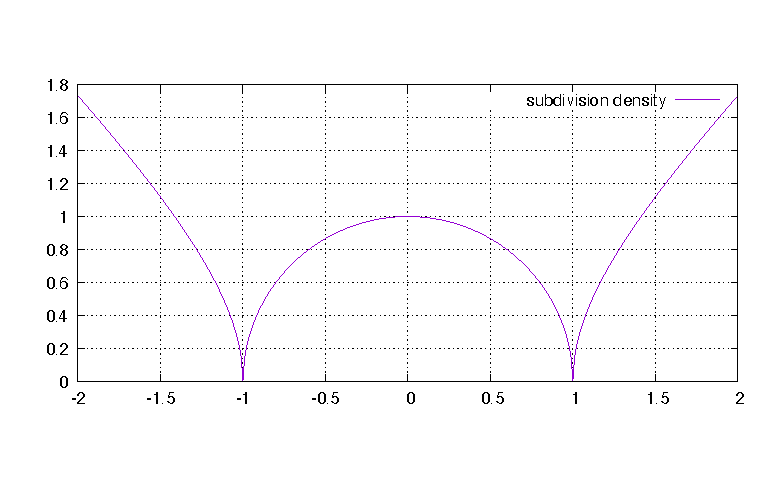
\includegraphics[scale=0.6]{subdiv_density}
    \caption{Subdivision density for the parallel curve of an Euler spiral}
    \Description{A graph of subdivision density. The range from -1 to 1 is a semicircle, and the value from 1 rises sharply from zero to an asymptote of unity slope.}
    \label{fig:subdiv_density}
\end{figure}

The subdivision density integral for the parallel curve of an Euler spiral is given as follows:

\[
    f(x) = \int_0^x\sqrt{|u^2 - 1|} du
\]

This integral has a closed-form analytic solution:

\[
    f(x) = \left\{
        \begin{array}{rl}
            \frac{1}{2}(x\sqrt{|x^2-1|} + \sin^{-1}x) & \text{if } |x| \leq 1 \\
            \frac{1}{2}(x\sqrt{|x^2-1|} - \cosh^{-1}x + \frac{\pi}{4}) & \text{if } x \geq 1
        \end{array}
    \right.
\]

Values for $x<-1$ follow from the odd symmetry of the function. 


\subsection{Approximation of the subdivision density integral}

The subdivision density integral [TODO: probably should use section or equation number reference] is fairly straightforward to compute in the forward direction, but not invertible using a straightforward closed-form equation. Numerical techniques are possible, but require multiple iterations to achieve sufficient accuracy, so are slower. In this subsection, we present a straightforward and accurate approximation, based on piecewise easily invertible functions. If higher flattening quality is desired at the expense of slower computation, this approximation can be used to determine a good initial value for numeric techniques; two iterations of Newton solving are enough to refine this guess to within 32-bit floating point accuracy.

The approximation is given as follows:

\[ 
    f_\mathit{approx}(x) = \left\{
        \begin{array}{rl}
            \frac{\sin c_1 x}{c_1} & \text{if } x < 0.8 \\
            \frac{\sqrt{8}}{3}(x-1)^{1.5} + \frac{\pi}{4} & \text{if } 0.8 \leq x < 1.25 \\
            0.6406x^2 - 0.81x + c_2 & \text{if } 1.25 \leq x < 2.1 \\
            0.5x^2 - 0.156x + c_3 & \text{if } x \geq 2.1
        \end{array}
        \right.
\]
\[
    \begin{array}{ll}
        c_1 = & 1.0976991822760038 \\
        c_2 = & 0.9148117935952064 \\
        c_3 = & 0.16145779359520596
    \end{array}
\]

The primary rationale for the constants is for the approximation to be continuous. The other parameters were determined empirically; further automated optimization is possible but is unlikely to result in dramatic improvement. Further, this approximation is given for positive values. Negative values follow by symmetry, as the function is odd.

The exact integral and the approximation given above are shown in Figure~\ref{fig:espc}. Visually, it is clear that the agreement is close, and in numerical testing the worst case discrepancy between approximate and exact results is approximately 6\%.

\begin{figure}
    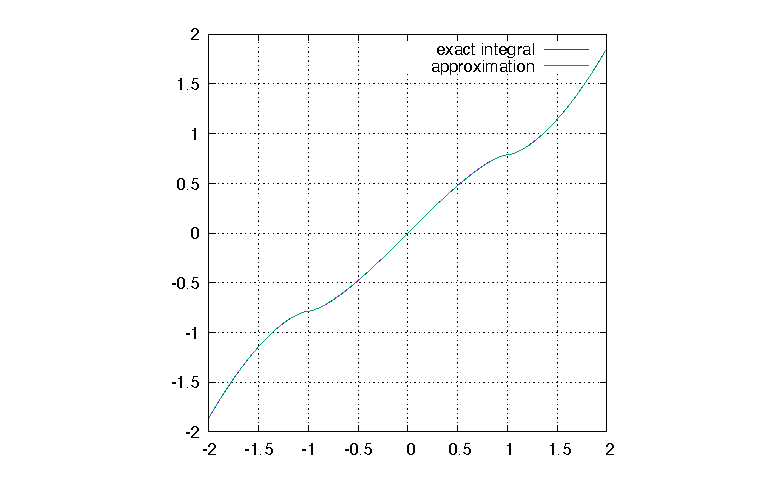
\includegraphics{espc}
    \caption{Integral of subdivision density for Euler spiral parallel curve, and its approximation}
    \Description{A graph of the integral of subdivision density. It is a wriggly diagonal line, with flat parts at -1 and 1. The approximation is nearly indistinguishable from the exact value.}
    \label{fig:espc}
\end{figure}

\section{Error metrics for approximation by arcs}

The problem of approximating a curve by a sequence of arc segments has extensive literature, but none of the published solutions are quite suitable for our application. The specific problem of approximating an Euler spiral by arcs is considered in \cite{Meek2004} using a ``cut then measure'' adaptive subdivision scheme, but their solution has poor quality; it scales as $O(1/n^2)$, while $O(1/n^3)$ is attainable. The result was improved ``slightly'' by \cite{Narayan2014}. The literature also contains optimal results, namely \cite{Maier2014} and \cite{Nuntawisuttiwong2021}, but at considerable cost; both approaches claim $O(n^2)$ time complexity. The through-line for all these results is that they are solving a harder problem: adopting the constraint that the generated arc sequence is $G^1$ continuous. While desirable for many applications, this constraint is not needed for rendering a stroke outline. Even with this constraint relaxed, the angle discontinuities of an arc approximation are tiny compared to flattening to lines.

% I also expect that the Fréchet distance error of a solution not constrained by G1 continuity will be better by some constant factor (somewhere around 2-4, just as a gut feeling) than the G1-continuous optimum solution. This is a major reason why we have such favorable segment counts, even in comparison to Euler spirals. However, providing evidence for that claim feels more in scope for another paper.

Our approach is based on a simple error metric, similar in flavor to the one for flattening to line segments. The details of the metric (in particular, tuning of constants) were obtained empirically, though we suspect that more rigorous analytic bounds could be obtained. In practice it works very well indeed; the best way to observe that is an interactive testing tool, which is provided in the supplemental materials.

The proposed error metric is as follows. The estimated distance error for a curve of length $\hat{s}$ is:

\[
    d \approx \frac{1}{120}\left(\int_0^{\hat{s}} \sqrt[3]{|\kappa'(s)|}ds \right)^3
\]

For an Euler spiral segment, $\kappa'(s)$ is constant and thus this error metric becomes nearly trivial. With n subdivisions, the estimated distance is simply $\frac{s^3\kappa'}{120n^3}$. Solving for $n$, we get $n = s\sqrt[3]{\frac{|\kappa'|}{120d}}$ subdivisions, and those are divided evenly by arc length, as the subdivision density is constant across the curve, just as is the case for flattening arcs to lines.

TODO: image. This will likely strongly resemble Fig. 8a from Narayan2014.

Remarkably, the approximation of an Euler spiral parallel curve by arc segments is almost as simple as that for Euler spirals to arcs. As in flattening to lines, the parameter for the curve is the arc length of the originating Euler spiral. The subdivision density is then constant, and only a small tweak is needed to the formula for computing the number of subdivisions, taking into account the additional curvature variation from the offset by $h$ (the half line-width). The revised formula is:

\[
    n = s\sqrt[3]{\frac{|\kappa'|(1+0.4|hs\kappa'|)}{120d}}
\]

This formula was determined empirically by curve-fitting measured error values from fitting Euler spiral parallel curves to arcs, but was also inspired by applying the general error metric formula to the analytical equations for Euler spiral parallel curve, and dropping higher order terms. A more rigorous derivation, ideally with firm error bounds, remains as future work.

One consequence of this formula is that, since $h$ appears under absolute value, the same arc approximation can be used for both sides of a stroke.

% Make improved quality claim here? I think it may be too subtle.

\section{Evolutes}

In the principled, correct specification for stroking\cite{Nehab2020}, parallel curves are sufficient only for segments in which the curvature does not exceed the reciprocal half width. When it does, additional segments must be drawn, including evolutes of the original curve. In general, the evolute of a cubic Bézier is a very complex curve, requiring approximation techniques. By contrast, the evolute of an Euler spiral ($\kappa = as$) is another spiral with a simple Cesàro equation, namely $\kappa = -a^{-1}s^{-3}$, an instance of the general result that the evolute of a log-aesthetic curve is another log-aesthetic curve\cite{Yoshida2012}.

Flattening this evolute is also straightforward; the subdivision density is proportional to $s^{-0.5}$ where $s$ is the arc length parameter of the underlying Euler spiral (and translated so $s = 0$ is the inflection point). Thus, the integral is $2\sqrt{s}$, and the inverse integral is just squaring. Thus, flattening the evolute of an Euler spiral is simpler than flattening its parallel curve.

\begin{figure}
    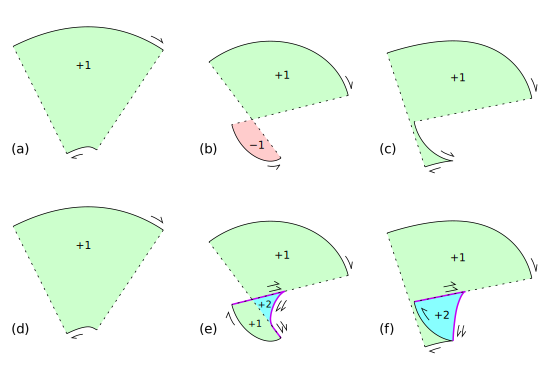
\includegraphics[scale=0.6]{evolute_fig}
    \caption{Weakly and strongly correct stroke outlines. The top row shows weakly correct stroke outlines. In (a) the curvature does not exceed the reciprocal half-width, and the stroke is rendered correctly. In (b) the curvature of the bottom outline consistently exceeds the reciprocal half-width, and a section of the outline incorrectly has negative winding number. In (c) there is a cusp. The bottom row shows corresponding strongly correct renders; (d) is the same as (a), while the other two show additional segments for the evolute and connecting lines (in purple). Note that the sections of parallel curve outline with above-threshold curvature are reversed, and that the section enclosed by the evolute has a total winding number of +2.}
    \Description{Two rows of rendered strokes, the top being weakly correct, only drawing parallel curves, the bottom being strongly correct, with additional evolute segments.}
    \label{fig:evolutes}
\end{figure}

The effect of adding evolutes to achieve strong correctness is shown in Figure~\ref{fig:evolutes}. The additional evolute segments and connecting lines are output twice, to make the winding numbers consistent and produce a watertight outline. All winding numbers are positive, so rendering with the nonzero winding number yields a correct final render.

\section{Conversion from cubic Béziers to Euler spirals}

The Euler spiral segment representation of a curve is useful for computing near-optimal flattened parallel curves, but standard APIs and document formats overwhelmingly prefer cubic Béziers as the path representation.

Many techniques for stroke expansion described in the literature apply some lowering of cubic Bézier curves to a simpler curve type, more tractable for evaluating parallel curve. Computing parallel curves directly on cubic Bézier curve segments is not very tractable. In particular, the widely cited Tiller-Hanson algorithm\cite{Tiller1984} performs well for quadratic Béziers but significantly worse for cubics.

% TODO: the discussion of adaptive subdivision maybe duplicates the earlier section on "measure then cut."

A typical pattern for converting from one curve type to another is \emph{adaptive subdivision.} (TODO: is there a good general reference for this?) An approximate curve is found in the parameter space of the target curve family. The error of the approximation is measured. If the error exceeds the specified tolerance, the curve is subdivided (typically at $t = 0.5$), otherwise the approximation is accepted. Subdivisions are also indicated at special points; for example, since quadratic Béziers cannot represent inflection points, and geometric Hermite interpolation is numerically unstable if the input curve is not convex, lowering to quadratic Béziers also requires calculation of inflection points and subdividing there. A good example of this pattern is Nehab\cite{Nehab2020}. One advantage of Euler spirals over quadratic Béziers is that they can represent inflection points just fine, so it is not necessary to compute those for additional subdivision.

The approach in this paper is another variant of adaptive subdivision, with two twists. First, it's not necessary to actually generate the approximate curve to measure the error. Rather, a straightforward closed-form formula accurately predicts it. The second twist is that, since compute shader languages on GPUs typically don't support recursion, the stack is represented explicitly and the conceptual recursion is represented as iterative control flow. This is an entirely standard technique, but with a clever encoding the entire state of the stack can be represented in two words, each level of the stack requiring a mere single bit.

\subsection{Error prediction}

A key step in approximating one curve with another is evaluating the error of the approximation. A common approach (used in \cite{Nehab2020} among others) is to generate the approximate curve, the measure the distance, often by sampling at multiple points on the curve. All this is potentially slow, with the additional risk of underestimating the error due to undersampling.

Our approach is different. In short, we perform a straightforward analytical computation to accurately estimate the error. Our approach to the error metric has two major facets. First, we obtain a cubic Bézier which is a very good fit to the Euler spiral, then we estimate the distance between that and the source cubic. Due to the triangle inequality, the sum of these is a conservative estimate of the true Fréchet distance between the cubic and the Euler spiral.

For mathematical convenience, the error estimation is done with the chord normalized to unit distance; the actual error is scaled linearly by the actual chord length.

The cubic Bézier approximating the Euler spiral is that with the distance of each control point from the endpoint is $d = \frac{2}{3(1 + \cos \theta)}$, where $\theta$ is the angle of the endpoint tangent relative to the chord. This is a generalization of the standard approximation of an arc. It should be noted that this is not in general the closest possible fit, but it is computationally tractable and has near-uniform parametrization. In general it has quintic scaling; if an Euler spiral segment is divided in half, the error of this cubic fit decreases by a factor of 32. A good estimate of this error is:

\[
    4.6255\times10^{-6}|\theta_0+\theta_1|^5 + 7.5\times10^{-3}|\theta_0+\theta_1|^2|\theta_0-\theta_1|
\]



The distance between two cubic Bézier segments can be further broken down into two terms; in most cases, the difference in area accurately predicts the Fréchet distance between the curves. Two cubic Béziers with the same area and same tangents tend to be relatively close to each other, but there is some error stemming from the difference in parametrization. Area of a cubic Bézier segment is straightforward to compute using Green's theorem:

\[
    a = \tfrac{3}{20}(2d_0\sin \theta_0 + 2d_1\sin \theta_1 - d_0 d_1\sin(\theta_0+\theta_1))
\]

The conservative Fréchet distance estimate is 1.55 the absolute difference in area between the source cubic and the Euler spiral approximation. The final term for imbalance is as follows, with $\bar{d}_0$ and $\bar{d}_1$ representing the distance from the endpoints of the Euler approximation and $d_0$ and $d_1$ the corresponding distance in the source cubic segment, as in the area calculation above:

\[
    (0.005|\theta_0+\theta_1| + 0.07|\theta_0 - \theta_1|)\sqrt{(\bar{d}_0 - d_0)^2 + (\bar{d}_1 - d_1)^2}
\]

The total estimated error is the sum of these three terms. We have validated this error metric in randomized testing. For values of $\theta$ between $0$ and $0.5$, and values of $d$ between $0$ and $0.6$, this estimate is always conservative, and it is also tight: over Bézier curves generated randomly with parameters drawn from a uniform distribution this range, the mean ratio of estimated to true error is 1.656.

A visualization of combined error metric is shown in Figure~\ref{fig:cubic_err}, comparing measured and approximate error for a slice of the parameter space, fixing the endpoint angles to 0.1 and 0.2, and varying the distance from both endpoints to the control point.

\begin{figure}
    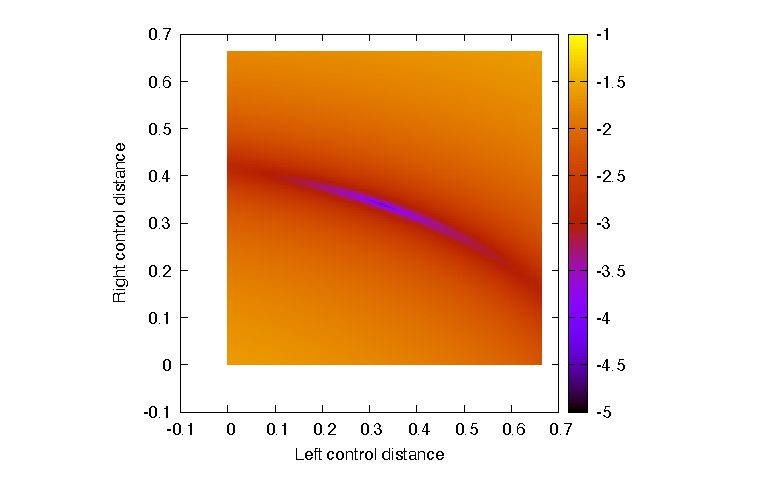
\includegraphics[scale=0.75]{cubic_err_measured} 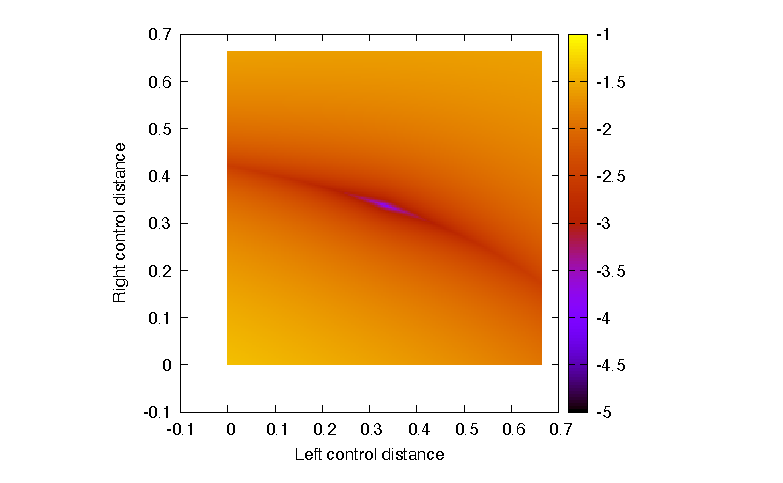
\includegraphics[scale=0.75]{cubic_err_approx}
    \caption{Comparision of measured (top) and approximated (bottom) error for cubic Bézier to Euler spiral conversion. Scale is log (base 10) of the error.}
    \Description{TODO}
    \label{fig:cubic_err}
\end{figure}

% Note about supplemental materials. This ratio is produced by examples/euler3 in Raph's local branch of euler_err_experiment of kurbo (git 99b00). This should be cleaned up and moved into the code repo.

\subsection{Geometric Hermite interpolation}

Given tangent angles relative to the chord, finding the Euler spiral segment that minimizes total curvature variation is a form of geometric Hermite interpolation. There are a number of published solutions to this problem, involving nontrivial numerical solving techniques: gradient descent\cite{Kimia2003}, bisection\cite{Walton2009}, or Newton iteration\cite{Connor2014}. A more direct approach is to approximate the function as a reasonably low-order polynomial in terms of the endpoint angles. Our approach is to use a 7th order polynomial, which is more precise than the 3rd order polynomial proposed in \cite{Reif2021}, at only modest increased cost. The exact coefficients used are presented in Appendix \ref{appendix:gh}.

\subsection{Unrolled recursion}

The entire recursion stack for adaptive subdivision can be represented in two words: dt and scaled\_t0. The range is dt * scaled\_t0 .. dt * (scaled\_t0 + 1). Initial values of 1 and 0 represent the range (0, 1). Pushing the stack, subdividing the range in half, is representing by halving dt and doubling scaled\_t0, which leaves the start of the range invariant but its size halved. After accepting an approximation, the next range is determined by incrementing scaled\_t0, then repeatedly popping the stack by doubling dt and halving scaled\_t0, as long as the latter is odd. This can in fact be achieved without iteration by using the ``count trailing zeros'' intrinsic.

\subsection{Cusp handling}

There are two types of cusps that must be handled in the stroke expansion problem. One is when the input cubic Bézier contains a cusp (or near-cusp, which is prone to numerical robustness issues), and one is when the parallel curve contains cusps. This section will describe both in order.

A Bézier curve is expressed in parametric form, and the derivative with respect to the parameter can be zero or nearly so, causing serious numerical problems for many stroke expansion algorithms. In the limit, as the Bézier curve describes a semi-cubical parabola, the curvature can become infinite.

Our approach is to leverage the conversion to Euler spiral segments, which have finite curvature. The geometric Hermite interpolation depends on accurate tangents at the endpoints, which in turn are derived from derivatives. The tangents are not well defined when the derivative is zero, and are not numerically stable when near-zero. Thus, the algorithm has one major mechanism to deal with numerical robustness in these cases: when sampling the cubic Bézier, if the derivative is near zero (as determined by testing against an epsilon threshold), then the derivative is sampled at a slightly perturbed parameter value.

In practice, when rendering a cubic Bézier with a cusp, the region near the cusp is rendered with one Euler spiral segment approximately in shape of the top of a question mark, as shown in Figure~\ref{fig:cusp_rendering}. Its parallel curve is well defined, and has the correct shape for the outline of the stroke, given of course that the distance is within tolerance (as enforced by the error metric).


\begin{figure}
    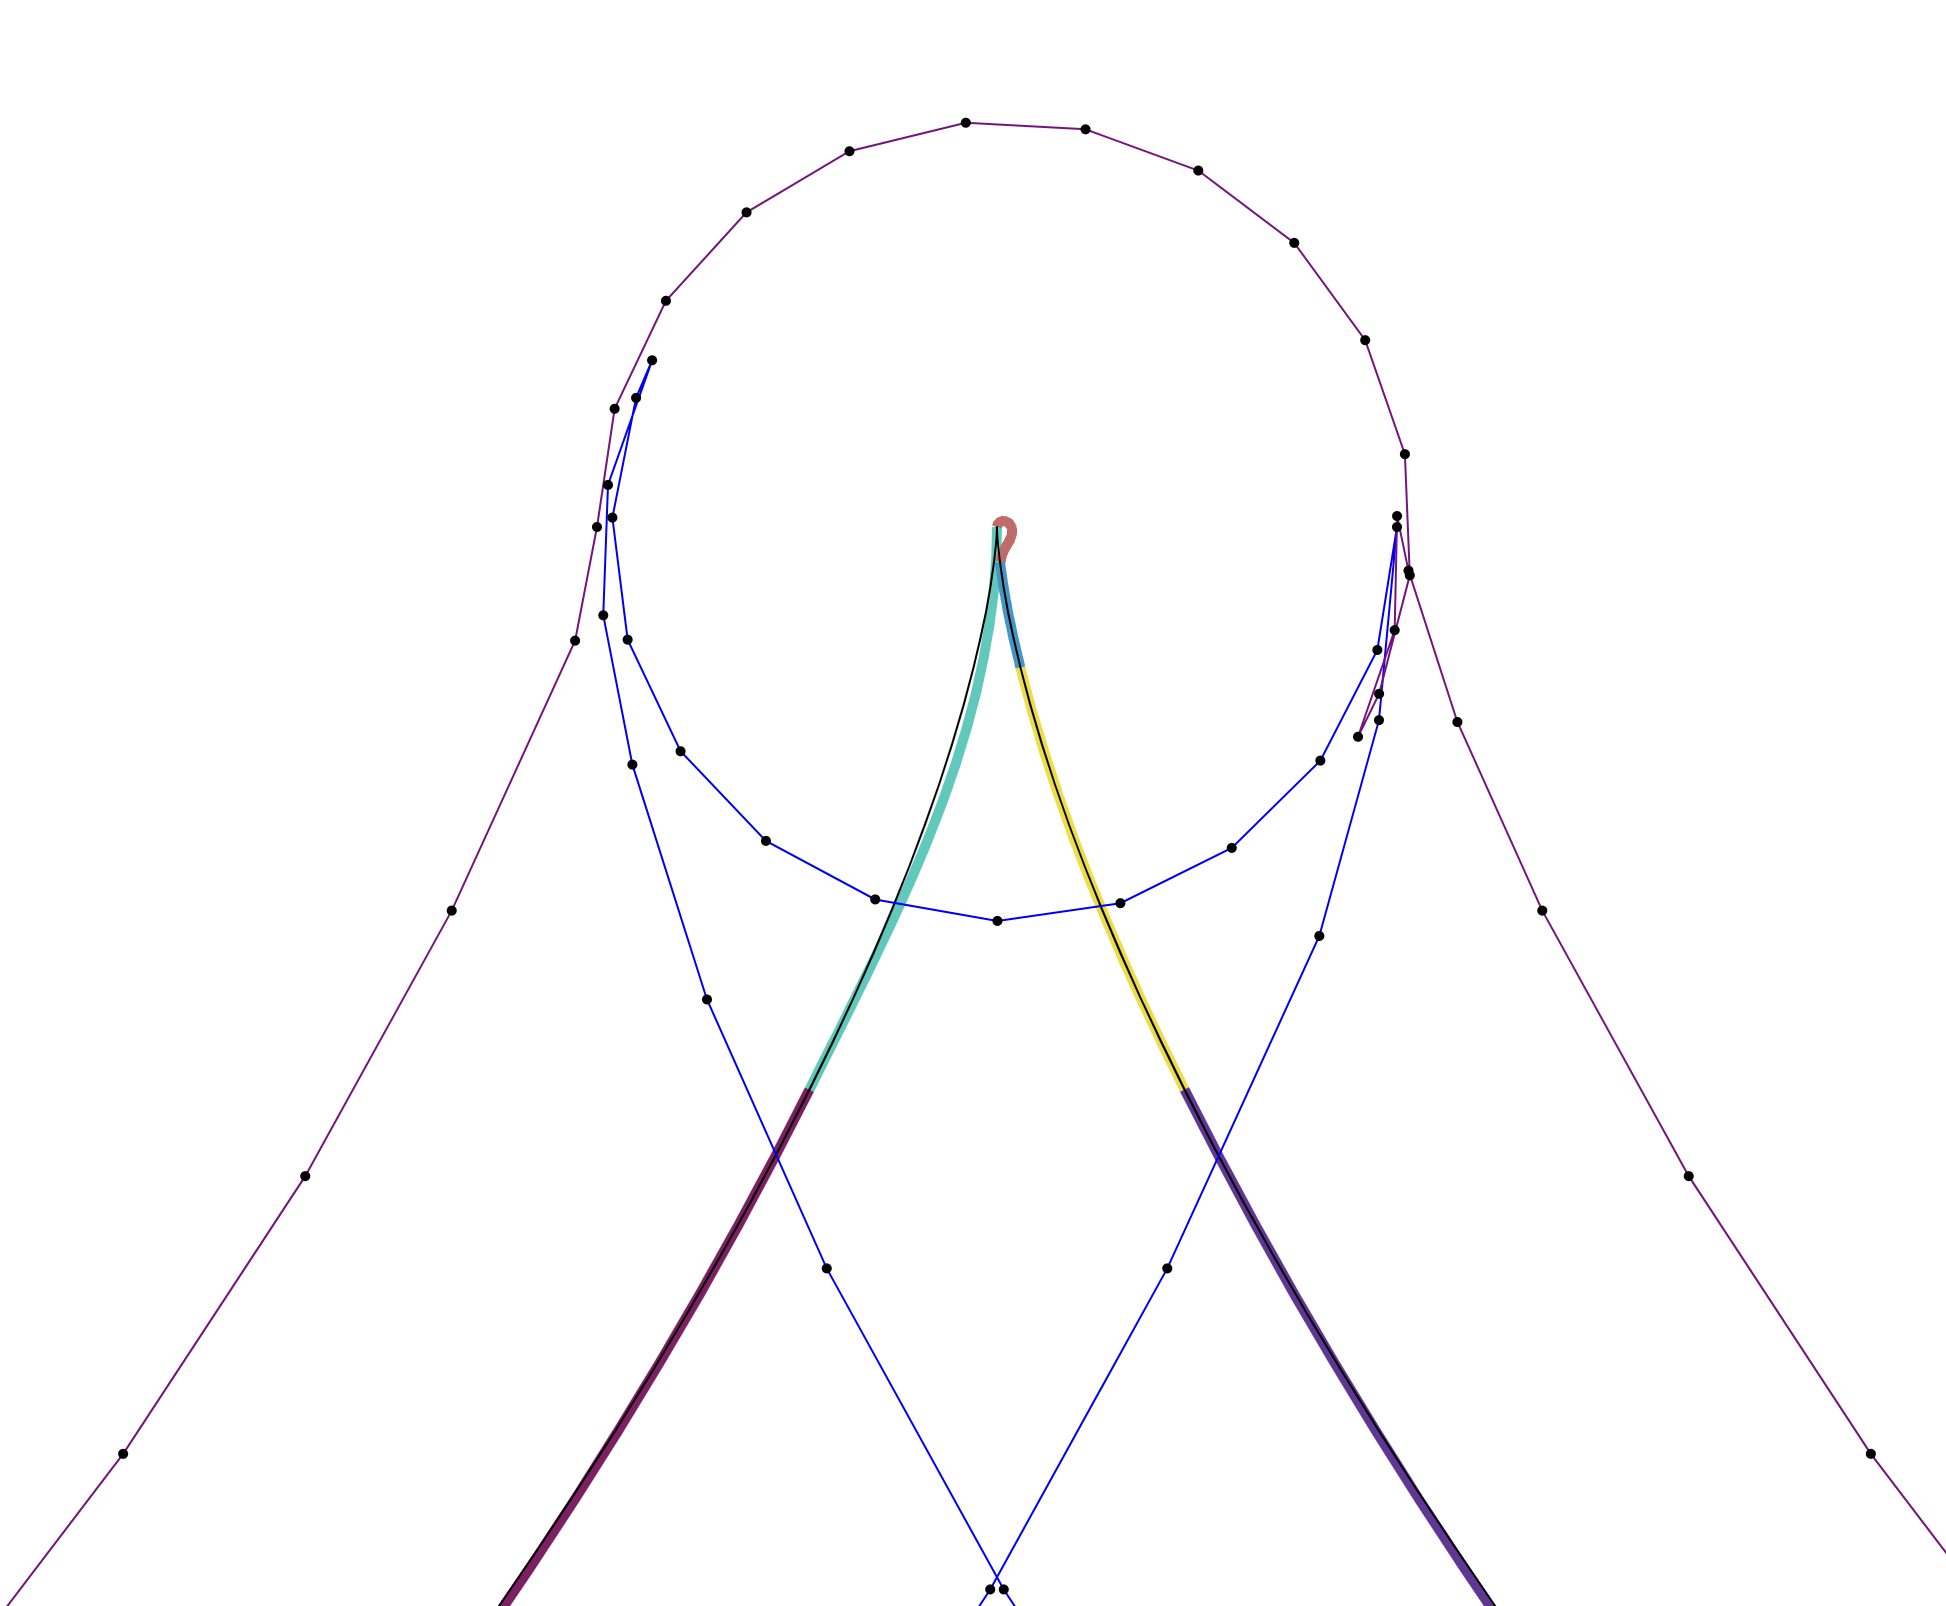
\includegraphics[scale=0.24]{cusp_rendering}
    \caption{Rendering of a cubic Bézier cusp using Euler spiral segments}
    \Description{A cubic Bézier with a cusp is approximated by Euler spiral segments with finite curvature, including one with a question mark shape. The resulting stroke outlines have the correct shape.}
    \label{fig:cusp_rendering}
\end{figure}

As recommended in both \cite{Nehab2020} and \cite{Kilgard2020}, the rendering of a cusp with infinite curvature matches that of a near-cusp. The code to detect near-zero derivatives and re-evaluate is a small amount of non-divergent logic, unlike the additional ``regularization'' pass proposed in Section 3.1 of \cite{Nehab2020} to handle special cases.

\subsubsection{Cusps in parallel curves}

Even when the input curve is smooth, its parallel curve contains a cusp when the (signed) curvature equals the offset distance (the half-width of the stroke). In published techniques, dealing with these cusps is a nontrivial effort, and involves numerical methods that are not GPU friendly. In particular, detecting locations in the cubic Bézier where the curvature crosses a given quantity is a medium-degree polynomial, and in general requires numerical techniques for root finding. In the approach of \cite{Nehab2020}, the root finder not only requires a hybrid Newton/bisection method, which requires iteration, but is also recursive in that it uses the roots of a polynomial of one degree lower as a subroutine. In general, polynomials up to cubic can be considered GPU-friendly, while finding cusps in cubic Béziers requires a higher degree.

In the simplest case, weak stroke correctness with line segments as the output primitive, no additional work is needed -- the flattening algorithm for Euler spiral parallel curves will naturally generate a point within the given error tolerance of the true cusp. However, generation of arc segments and drawing the evolutes needed for strong correctness both require subdivision at the parallel curve cusps.

Fortunately, finding the cusp in the parallel curve of an Euler spiral parallel curve is a simple linear equation, and there is at most one cusp in any such segment. Euler spirals are thus a good solution for determining cusps as a piecewise linear approximation to curvature.

\section{GPU Implementation} \label{section:gpu-impl}

We applied the techniques outlined in Section 7 to implement a data-parallel algorithm that can convert stroked 2D Bézier paths into flat geometry suitable for GPU rendering. We focused primarily on the global stroke-to-fill conversion problem in order to generate polygonal outlines for rasterization. Since the Euler spiral approximation can fit any source cubic Bézier and its parallel offset curves, our implementation can be used to render both filled and stroked primitives within a satisfactory error tolerance.

We aimed to satisfy the following the criteria:
\begin{enumerate}
  \item The implementation must be able to handle a large number of inputs at real-time rates. 
  \item The stroke outlines must meet the weak correctness definition.
  \item The implementation must support the standard SVG stroke end cap (\emph{butt}, \emph{square}, \emph{round}) and join styles (\emph{bevel}, \emph{miter}, \emph{round}).
  \item The CPU must do no work beyond the basic preparation of the input path data for GPU consumption.
\end{enumerate}

One of our artifacts is a GPU compute shader that satisfies these criteria. We coupled this with a simple and efficient data layout for parallel processing. Notably, our implementation is fully data-parallel on input path segments and does not require any computationally expensive curve evaluation on the CPU. We implemented our shader on general-purpose GPU compute primitives supported by all modern graphics APIs, particularly Metal, Vulkan, D3D12, and WebGPU[? citation?]. As such, the ideas presented in this section are portable to various GPU platforms.

The rest of this section describes the design of our GPU pipeline and input encoding scheme.

% TODO: - Watertightness

\subsection{Pipeline Design} \label{subsec:pipeline-design}

An SVG path consists of a sequence of instructions (or "verbs"). The \emph{lineto} and \emph{curveto} instructions denote an individual \emph{path segment} consisting of either a straight line or a cubic Bézier. A given subsequence of path segments can be bounded by a \emph{moveto} and/or \emph{closepath} instruction which mark the beginning and end of a \emph{subpath}. A subpath must form a closed contour if painted as a fill. When painted as a stroke, each subpath must begin and end with a cap according to the desired cap style. In addition, each path segment in a stroked subpath must be connected to adjacent path segments of the same subpath with a join. For any given path, the cap and join styles do not vary across subpaths or individual path segments.

The standard organizational primitive for a compute shader is the \emph{workgroup}. A workgroup can be organized as a 1, 2, or 3-dimensional grid of individual threads that can cooperate using shared memory. Multiple workgroups can be \emph{dispatched} as part of a larger global grid, also of 1, 2, or 3 dimensions.

Our compute shader is arranged as a 1-dimensional grid, parallelized over input path segments. We chose a workgroup size of 256 as it works well over a wide range of GPUs. However, this choice of workgroup size is not particularly important for our algorithm as it does not require any cross-thread communication. Each thread in the global grid is assigned to process a single path segment. We encode the individual path segments contiguously in a GPU storage buffer such that each element has 1:1 correspondance to a global thread ID in the dispatch. This layout easily scales to hundreds of thousands of input path segments, which can be distributed across any number of paths and subpaths. We submit the kernel to the GPU as a single dispatch with as many workgroups as needed to handle the entire input.

\begin{center}
\begin{figure}
    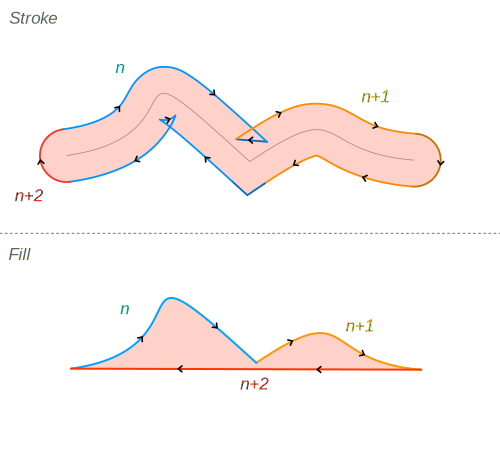
\includegraphics[scale=0.18]{stroke_threads}
    \caption{Visualization of contour outlines and the IDs of GPU threads that flatten them. The subpath contains two adjacent cubic Bézier curves rendered as both a stroke and a fill. In the stroked version, thread $n$ flattens the offset curves of the first curve (blue) and the join segment with the miter style (dark blue). Thread $n + 1$ flattens the offset curves of the second curve (orange) and the end cap with the round style (dark orange). Thread $n + 2$ handles the \emph{subpath end segment} and flattens the start cap (red). When the same path is rendered as a fill, threads $n$ and $n + 1$ each flatten the source curves, while thread $n + 2$ outputs the \emph{close} segment that joins the end of the subpath to its starting point. The black arrows represent the winding direction of the output segments.}
    \Description{TODO}
    \label{fig:stroke_threads}
\end{figure}
\end{center}

\begin{algorithm}
  $tid \gets$ global invocation ID\;
  $(style, segment) \gets readScene(tid)$\;
  \eIf{$style$ is $fill$}{
      output source curve\;
  }{
      \tcp{Handle stroked segment}
      \eIf{$segment$ is \emph{stroke cap marker}}{
          \eIf{path is open}{output start cap\;}{output nothing\;}
      }{
          output both offset curves\;
          $neighbor \gets readScene(tid + 1)$\;
          \eIf{$neighbor$ is not \emph{stroke cap marker} OR path is closed}{
              output join\;
          }{
              output end cap\;
          }
      }
  }
\caption{The control flow of the compute shader}
\label{alg:shader-flow}
\end{algorithm}

Each thread outputs a polyline that fits a subset of the rendered subpath's outer contour, represented by the path segment (see Figure \ref{fig:stroke_threads}). For a filled primitive, a thread only outputs the flattened approximation of the path segment. For a stroke, a thread outputs the polylines approximating multiple curves: a) the two parallel curves on both sides of the source segment, offset by the desired stroke \emph{halfwidth}, and b) the joins that connect the path segment to the next adjacent segment. We also store metadata in our input encoding that marks the position of a path segment within the containing subpath. We use this information to determine whether to output an end cap instead of a join. We encode one additional segment designated as the \emph{stroke cap marker} for every subpath. The thread assigned to the marker segment only outputs a start cap, which completes the stroke outline.

The joins between adjacent segments need to form a continuous outline when combined with the segments. This requires that a thread have access to the tangent vector at the end of its assigned segment \emph{and} the start tangent of the next adjacent segment. We require that the input segments within a subpath are stored in order which simplifies the access to the adjacent segment down to a buffer read at the next array offset. While we take care to output the \emph{outer} join segment (where the offset curves meet at a reflex angle) according to the join style, we output the inner join simply as a line segment.

A property of this data-parallel structure is that the output is unordered. The cubic-Bézier-to-Euler-spiral conversion is sequential within a single thread, so it is possible to preserve ordering at the scope of an individual path segment, if desired. However, ordering cannot be guaranteed across path segments. We refer to this output data structure as \emph{line soup}. We integrated the compute shader as a stage in a larger compute shader pipeline (discussed in Section \ref{subsection:gpu-results}) that spatially sorts the line soup in subsequent binning and tiling stages prior to rasterization.

The compute shader writes the line soup output to a GPU storage buffer. Each line soup entry contains the viewport coordinates of the two endpoints of a singe line segment. We also implemented a variant that outputs circular arc segments instead of lines, in which the output entries contain the arc endpoints in addition to its curvature. For both primitive types, our renderer also outputs a 32-bit \emph{path ID} used by downstream pipeline stages to identify the path that a segment belongs to, in order to retrieve the correct paint (solid or gradient color) for rendering.

\subsection{Input encoding}

The input to our pipeline consists of a sequence of paths, each with an associated 2D affine transformation matrix and a \emph{style} data structure containing information about the stroke style or fill rule. We encode paths, transforms, and styles as parallel input streams. Unlike a conventional structure-of-arrays arrangement, we permit a one-to-many mapping across elements between certain streams: each transform and style entry can apply to one or more path entries with an array index greater than or equal to transform or style index.

Paths get encoded as two parallel streams: a \emph{path tag} stream containing an element for every segment in every subpath, and a \emph{path data} stream of point coordinates. Each segment/verb contributes a variable number of points: 1 for \emph{moveto}/\emph{lineto}, 2 for quadratic Béziers, and 3 for cubic Béziers. This variable length stream encoding allows for a highly compact representation of SVG-type content in memory. A GPU thread assigned to a path segment must be able to reference the corresponding element in each stream in order to obtain the right curve coordinates, transform, and style information. This is done by computing a set of stream offsets for every element in the path tag stream.

% TODO: Figure: streams and tagmonoid relationship, plus sizes of the elements, plus monoid bits

We compute the offsets on the GPU in a separate compute shader that runs prior to the flattening stage. A path tag consists of 8 bits that store \emph{stream offset increments}, such that the inclusive prefix sums of all increments for every element in the tag stream yield the stream offsets. We call this structure the \emph{tag monoid} and have implemented the computation as a general parallel prefix scan.[TODO: citation?]

\begin{table}
    \caption{
        \emph{Coordinate count} indicates the type of path segment: 1 for lines, 2 for quadratic Béziers, 3 for cubic Béziers. The \emph{subpath end bit} is set on the last segment of a subpath and the \emph{path bit} is additionally set on the last tag of a path. The number of curve control points is given by \emph{coordinate count}, plus $1$ if the subpath end bit is set. The number of bytes per coordinate pair is 4 for 16 bit or 8 for 32 bit coordinates.
    }
    \begin{tabular}{|c|l|}
    \hline
        \textbf{Path Tag Bits} & \multicolumn{1}{|c|}{\textbf{Monoid Fields}} \\
    \hline
        0-1 & coordinate count \\
        2 & subpath end bit \\
        3 & 16/32 bit coordinates \\
        4 & path bit \\
        5 & transform bit \\
        6 & style bit \\
    \hline
    \end{tabular}
    \label{table:pathtag}
\end{table}

Table~\ref{table:pathtag} shows the individual fields of the 8-bit path tag. The offset increments for the transform and style streams can be stored in a single bit that is set to $1$ only if a path tag marks the beginning of a new transform and/or style entry. We also encode an additional \emph{path bit} in the final segment of all paths, which allows us to access additional streams (such as fill color or gradient parameters) using a per-path offset in later rendering stages.

The handling of the subpath bit allows for overlap in coordinates, so that except at subpath boundaries, the first coordinate pair of each segment overlaps with the last coordinate pair of the previous one. During the CPU-side encoding, subpath boundaries are moved from the beginning of a subpath (moveto) to the end. The encoding process inserts an additional line segment into the tag and coordinate streams to close the subpath if the final point does not coincide with the start point. The \emph{subpath end bit} is set to $1$ for the final segment of every subpath. For strokes, the subpath end segment represents the \emph{stroke cap marker} defined in Section \ref{subsec:pipeline-design}. This special segment is assigned a coordinate count of $2$, and the corresponding two points in the path data stream encode the tangent vector of the subpath's initial segment, used to correctly draw the start cap or the connecting join in a closed contour.

\subsection{Flattening Algorithm}

% TODO: explain flatten_euler
% TODO: visualize per-segment flattened output for a fill and for a stroke from the perspective of one thread.

% TODO: memory usage discussion: the impact of lines and how arcs might help. or work graphs, or maybe mesh shaders. Limitation: memory must be allocated up-front. bump estimation, violates the no pre-curve-evaluation criterium but simpler techniques (like Wang's) exist and we use it but way over-estimates. This is a limitation of the GPU execution model. Explain this trade-off.
  % -> TODO: Memory usage graphs for input scene buffers and LineSoup.
% TODO: pathological cases: our implementation doesn't handle culling.

\section{Results}

% TODO: discuss: divergence (reference prim count)

We present two versions of our stroking method: a sequential CPU stroker and the GPU compute shader outlined in Section \ref{section:gpu-impl}. Both versions can generate stroked outlines with line and arc primitives. We focused our evaluation on the number of output primitives and execution time, using the \emph{timings} dataset provided by Nehab2020\cite{Nehab2020}, in addition to our own curve-intensive scenes to stress the GPU implementation. We presents our findings in the remainder of this section.

\subsection{CPU: Primitive Count and Timing}

We measured the timing of our CPU implementation, generating both line and arc primitives, against the Nehab and Skia strokers, which both output a mix of straight lines and quadratic Bézier primitives. The results are shown in Figure~\ref{fig:timings}. The time shown is the total for test files from the \emph{timings} dataset of \cite{Nehab2020}, and the tolerance was 0.25 when adjustable as a parameter.

Similarly to \cite{Nehab2020}'s observations, Skia is the fastest stroke expansion algorithm we measured. The speed is attained with some compromises, in particular an imprecise error estimation that can sometimes generate outlines exceeding the given tolerance. We confirmed that this behavior is still present. The Nehab paper proposes a more careful error metric, but a significant fraction of the total computation time is dedicated to evaluating it.

\begin{figure}
    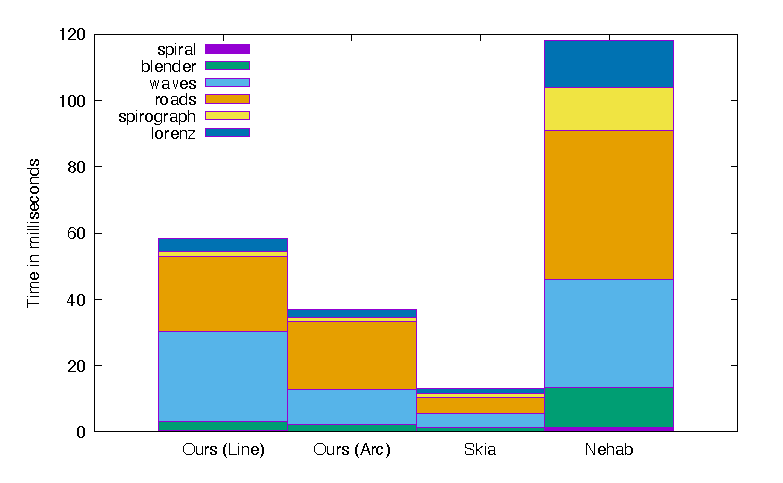
\includegraphics[scale=0.6]{timings}
    \caption{CPU timings for stroke expansion, comparing two versions of our stroker (outputting line and arc primitives) against Skia's curve-to-curve stroker. Measured on an AMD 3970}
    \Description{A stacked bar chart of the timings for stroke expansion}
    \label{fig:timings}
\end{figure}

We also compared the number of primitives generated, for varying tolerance values from 1.0 to 0.001. The number of arcs generated is significantly less than the number of line primitives. The number of arcs and quadratic Bézier primitives is comparable at practical tolerances, but the count of quadratic Béziers becomes more favorable at finer tolerances. The vertical axis shows the sum of output segment counts for test files from the \emph{timings} dataset, plus mmark-70k (as described in more detail in Section~\ref{subsection:gpu-results}), and omitting the \emph{waves} example\footnote{The \emph{waves} example triggers triggers Skia issue 336617138 at finer tolerance.}.

\begin{figure}
    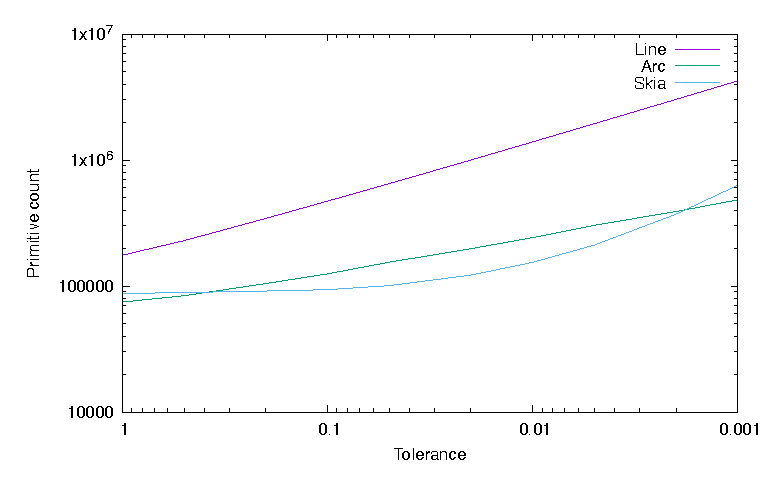
\includegraphics[scale=0.6]{prim_count}
    \caption{Primitive count for stroke expansion}
    \Description{A line chart showing the primitive count}
    \label{fig:prim_count}
\end{figure}

NOTE: the increase in Skia numbers at tolerances below 0.01 or so is the result of a precision bug in Skia, uncovered during preparation of this chart. We expect that to be fixed, and will revise the chart.

\subsection{GPU: Execution Time} \label{subsection:gpu-results}

We evaluated the runtime performance of our compute shader on 4 GPU models and multiple form factors: Google Pixel 6 equipped with the Arm \emph{Mali-G78 MP20} mobile GPU, the Apple \emph{M1 Max} integrated laptop GPU, as well as two discrete desktop GPUs: the mid-2015 NVIDIA {GeForce GTX 980Ti} and the late-2022 NVIDIA {GeForce RTX 4090}. We authored our entire GPU pipeline in the \emph{WebGPU Shading Language} (WGSL) and used the \emph{wgpu}\cite{wgpu} framework to natively interoperate with the native graphics APIs (we tested the M1 Max on macOS via the Metal API; the mobile and desktop GPUs were tested via the Vulkan API on Android and Ubuntu systems).

We instrumented our pipeline to obtain fine-grained pipeline stage execution times using the GPU \emph{timestamp query} feature supported by both Metal and Vulkan. This allowed us to collect measurements for the curve flattening stage in isolation. We ran the compute pipeline on the \emph{timings} SVG files provided by Nehab\cite{Nehab2020}. The largest of these SVGs is \emph{waves} (see rendering \emph{(a)} in Figure \ref{fig:renderings}) which contains 42 stroked paths and a total of 13,308 path segments.

In order to stress the GPU with a higher workload, we made two additional test scenes. The first is a very large stroked path with 503,304 individually styled dashed segments which we adapted from Skia's open-source test corpus. We used two variants of this scene with \emph{butt} and \emph{round} cap styles. For the second scene we adapted the \emph{Canvas Paths} test case from MotionMark\cite{todo:mmark}, which renders a large number of randomly generated stroked line, quadratic, and cubic Bézier paths. We made two versions with different sizes: mmark-35k and mmark-60k with 30,000 and 60,000 paths respectively. Table \ref{table:bump-counts} shows the payload sizes of our largest test scenes.

\begin{table}
    \caption{Comparison of input and output segment counts in the more intensive GPU test cases. \emph{Segments} are input path segments. \emph{Lines} and \emph{Arcs} are the output primitives.}
    \begin{tabular}{|l|c|c|c|}
    \hline
        \multicolumn{1}{|c|}{\textbf{Test}} & \textbf{Input Segments} & \textbf{Lines} & \textbf{Arcs} \\
    \hline
        waves.svg & 13,308 & 406,059 & 111,965 \\
        mmark-35k & 105,022 & 1,039,899 & 500,351 \\
        mmark-60k & 179,929 & 1,784,896 & 858,162 \\
        long dash (butt) & 503,304 & 1,060,476 & 1,060,476 \\
        long dash (round) & 503,304 & 2,013,216 & 1,060,476 \\
    \hline
    \end{tabular}
    \label{table:bump-counts}
\end{table}

The test scenes were rendered to a GPU texture with dimensions 2088x1600. The contents of each scene were uniformly scaled up (by encoding a transform) to fit the size of the texture, in order to increase the required number of output primitives. As with the CPU timings, we used an error tolerance of 0.25 in all cases. We recorded the execution times across 3,000 GPU submissions for each scene.

\begin{figure}
    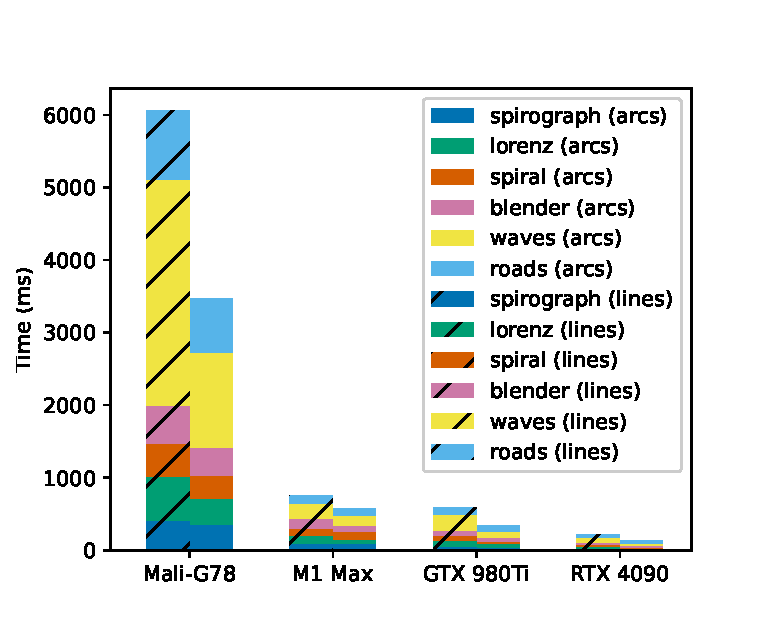
\includegraphics[scale=0.69]{nehab_gpu_timings}
    \caption{Mean GPU execution times of the compute shader that performs stroke expansion and flattening when run on the Nehab\cite{Nehab2020} \emph{timings} data set, in microseconds. The hatched bars show the timings for the version that outputs line primitives while the solid bars show that for arcs. Mali-G78 (the lowest end GPU we tested) converts \emph{waves} (the largest scene in the set) to lines in ~3ms. The compute shader executes at least an order of magnitude faster on the other GPUs.}
    \Description{A stacked bar chart of the GPU timings for stroke expansion from Nehab\cite{Nehab2020} timings SVGs}
    \label{fig:nehab-gpu-timings}
\end{figure}

\begin{figure}
    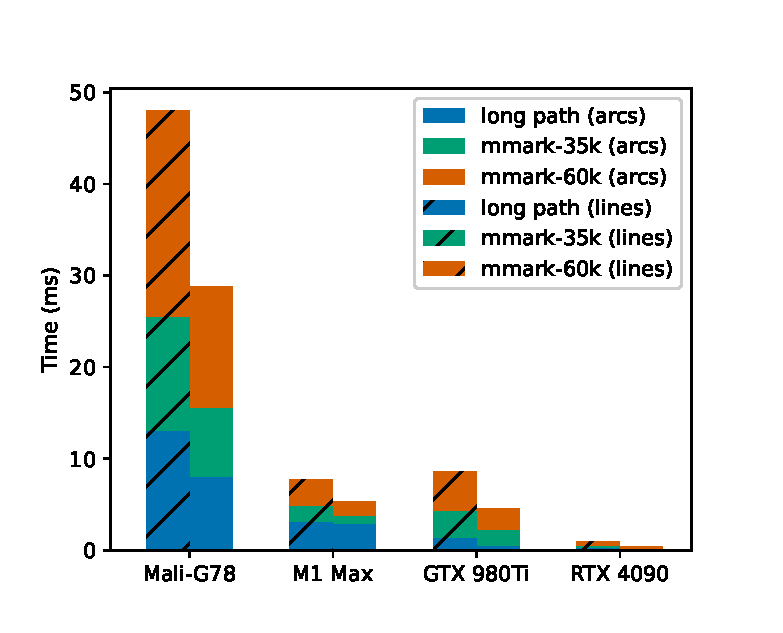
\includegraphics[scale=0.73]{test_scenes_gpu_timings}
    \caption{Mean GPU execution times of the compute shader that performs stroke expansion and flattening when run on the stress test scenes. The timings are shown in milliseconds.}
    \Description{A stacked bar chart of the GPU timings for stroke expansion from our test scenes}
    \label{fig:test-scenes-gpu-timings}
\end{figure}

\begin{figure*}
    \centering
    \includegraphics[scale=0.2]{test_renderings}
    \caption{Renderings of some of our test scenes created using our algorithm and associated frame rates. All images were rendered on an Apple M1 Max at 2088x1600 resolution using our GPU pipeline. \textbf{(a)} \emph{waves.svg} from the Nehab2020 timings data set (340fps); \textbf{(b)} The \emph{mmark-60k} scene with ~180k input segments (72fps); \textbf{(c)} The \emph{long path} scene with ~500k input segments and round caps (40fps with CPU-side dashing - the GPU time to render the scene is 9ms); \textbf{(d)}; A simple test scene showcasing various cap and join styles (950fps); \textbf{(e)} The famous \emph{Ghostscript Tiger} containing both stroked and filled paths (810fps).}
    \Description{Renderings of the test scenes}
    \label{fig:renderings}
\end{figure*}

Figures \ref{fig:nehab-gpu-timings} and \ref{fig:test-scenes-gpu-timings} show the execution times of our compute shader.
TODO: brief assessment.


% TODO: line soup is bump allocated. talk about allocation and estimation.

\section{Discussion}
\subsection{Limitations}

\section{Future work}

\begin{itemize}
    \item The GPU implementation sequentializes some work that could be parallel, and is thus not as well load-balanced as it might be. An appealing future direction is to split the pipeline into separate stages, executed by the GPU as nodes in a work graph\cite{Patel2024}. This structure is appealing because load balancing is done by hardware.

    \item Many of the error metrics were empirically determined. The mathematical theory behind them should be developed more rigorously, and that process will likely uncover opportunities to fine-tune the technique.
\end{itemize}

% TODO: mention dashing as future work? raph@: I think so. When we describe dashing, it would be good to say that the ES representation is already optimal for dashing, as it's parametrized by arc length.
% TODO: triangles

% TODO: while parallel on input, sequential per curve. However iterations are bounded (? needs measurement). Should this discussion happen here or down in the Performance section?
%    raph@: I don't have strong feelings on where the discussion happens. However, we want to make the following points:
%         * The concept is currently sequential only for cubic->ES, all else is parallelizable
%         * The current impl is sequential per curve, but that's just an impl choice. Personally I'm a fan of discussing this in future work related to work graphs, as I consider load balancing to be a detail
%         * Parallel lines per ES makes sense but parallel arcs per ES much less so, just because of the prim count. Thus, such detailed discussion may make sense downstream of the prim count results.

\bibliographystyle{ACM-Reference-Format}
\bibliography{paper}

\appendix

\section{Geometric Hermite interpolation for Euler spiral}
\label{appendix:gh}

This appendix gives the detailed algorithm for Geometric Hermite interpolation, determining Euler spiral segment parameters given the tangent angles at the endpoints relative to the chord.

The Euler spiral is represented by $\kappa(s) = k_0 + k_1s$, where $s$ ranges from 0 to 1, i.e. the arc length is unit normalized. This segment is scaled, rotated, and translated into place so that its endpoints match the desired locations. Immediately, $k_0$ can be determined as $\theta_0 + \theta_1$. Therefore, the remaining parameters to compute are $k_1$ and the ratio of chord length to arc length. The latter \emph{could} be computed from $k_0$ and $k_1$ by numerical integration, but it is more efficient to obtain it at the same time as $k_1$. Setting $k = \theta_0 + \theta_1$ and $\Delta = \theta_1 - \theta_0$, we have:

\[
    \setlength\arraycolsep{2pt}
    \begin{array}{rl}
    k_1 = & 6\Delta \\
     - & \Delta^3 / 70 \\
     - & \Delta^5 / 10780 \\
     + & \Delta^7 \cdot 2.769178184818219\times 10^{-7} \\
     - & k^2\Delta / 10 \\
     + & k^2\Delta^3 / 4200 \\
     + & k^2\Delta^5 \cdot 1.6959677820260655\times 10^{-5} \\
     - & k^4\Delta / 1400 \\
     + & k^4\Delta^3 \cdot 6.84915970574303\times 10^{-5} \\
     - & k^6\Delta \cdot 7.936475029053326\times 10^{-6}
    \end{array}
\]

Similarly, the formula for the chord to arc length ratio:

\[
    \setlength\arraycolsep{2pt}
    \begin{array}{rl}
    c = & 1 \\
    - & \Delta^2 / 40 \\
    + & \Delta^4 \cdot 0.00034226190482569864 \\
    - & \Delta^6 \cdot 1.9349474568904524\times 10^{-6} \\
    - & k^2 / 24 \\
    + & k^2\Delta^2 \cdot 0.0024702380951963226 \\
    - & k^2\Delta^4 \cdot 3.7297408997537985\times 10^{-5} \\
    + & k^4 / 1920 \\
    - & k^4\Delta^2 \cdot 4.87350869747975\times 10^{-5} \\
    - & k^6 \cdot 3.1001936068463107\times 10^{-6}
    \end{array}
\]

Note that the latter quantity is equal to $\mbox{sinc}(k/2)$ when $\Delta = 0$.

The coefficients were determined by numerical differentiation, using a Newton-style solver as the source of truth. The resulting formulas are extremely accurate over a wide range of inputs.

% TODO: we can definitely quantify that more precisely.

\end{document}
